\documentclass[]{scrartcl}
\usepackage{graphicx}
\usepackage{color}
\usepackage[ngerman]{babel}
\usepackage{hyperref}
\usepackage{fullpage}
\usepackage{calc} 
\usepackage{enumitem}
\usepackage{titlesec}
\newcommand{\todo}[1]{\textcolor{red}{TODO: #1}\PackageWarning{TODO:}{#1!}}
\begin{document}

\title{
	\includegraphics*[width=0.75\textwidth]{images/hu_logo.png}\\
	\vspace{24pt}
	Einf"uhrung in die Sprachphilosophie}
\subtitle{VEV WS 16/17\\
          Dr. Jasper Liptow\\
          Philosophisches Institut I \\ 
          Humboldt Universit"at zu Berlin}
\author{Lennard Wolf\\
        \href{mailto:lennard.wolf@student.hu-berlin.de}{lennard.wolf@student.hu-berlin.de}}
\maketitle
\begin{abstract}

Die Vorlesung soll grundlegendes Wissen "uber Probleme, Begriffe und Positionen der Sprachphilosophie des 20. Jahrhunderts vermitteln. Nach einer einf"uhrenden Einheit, in der das Ph"anomen der sprachlichen Bedeutung, das im Mittelpunkt sprachphilosophischer Untersuchungen steht, herausgearbeitet wird, widmen wir uns ausgew"ahlten systematischen Themen (wie etwa den verschiedenen Dimensionen sprachlicher Bedeutung, dem Zusammenhang von Bedeutung und Gebrauch sprachlicher Ausdr"ucke oder dem Verh"altnis von Sprache und Denken). Die Vorlesung wird von Tutorien begleitet, in denen Texte besprochen werden, die f"ur die Vorlesung eine Rolle spielen, und Fragen der Vorlesung vertieft diskutiert werden k"onnen.


\end{abstract}
\newpage

\tableofcontents
\listoffigures
\newpage


\section{Einf"uhrungssitzung\\(24.10.16)}
\subsection{Organisatorisches}

\begin{itemize}
  \item Jede Woche begleitender Text der vorher zu lesen ist (bis 30.11. k"onnen runtergeladen werden)
  \item In Tutorien werden Texte nachbesprochen
  \item 4 Essays (3-4 Standardseiten) f"ur Tutorien zum Bestehen 
  \item Passwort: Platte
\end{itemize}

\subsection{Was ist Sprachphilosophie?}
\subsubsection{Die Methode der Sprachphilosophie}

Ziel der Sprachphilosophie ist es, Erkenntnisse "uber Sprache zu gewinnen, ohne Empirie anzuwenden. Dadurch sollen philosophische Fragen \emph{verschwinden}. Unterschiede zu Empirischer Forschung sind umstritten, und diese k"onnen in den folgenden zwei Weisen betrachtet werden.

\textbf{Unterschiede prinzipieller Natur:} Empirische Wissenschaft untersucht die Welt \emph{direkt}, Philosophie durch eine Analyse unserer Begriffe | Art der Rechtfertigung: \emph{a priori} vs. \emph{a posteriori} | Art der Belege: Erfahrung vs. Intuition | Modaler Status des Wissens: kontingente Wahrheiten (Empirie) vs. notwendige Wahrheiten (Philosophie).

\textbf{Unterschiede gradueller Natur:} `Abstraktheit': Philosophie untersucht besonders abstrakte oder allgemeine Aspekte ihres Gegenstands | `Semantischer Aufstieg': Philosophische Untersuchungen reflektieren in einem besonderen Ma\ss e über den Gehalt der Begriffe, mit denen sie operieren | Bezug zu `allt"aglichem Selbstverst"andnis': Philosophische Erkenntnisse bleiben an unser allt"agliches
Selbstverst"andnis zur"uckgebunden | Reflexion auf Zusammenh"ange: Philosophische Untersuchungen reflektieren in besonderer Weise darauf, wie ihre Gegenst"ande mit Gegenst"anden anderer Bereiche zusammenh"angen.


\subsubsection{Der Gegenstand der Sprachphilosophie}

Der zentrale Gegenstand der Sprachphilosophie ist das Ph"anomen der sprachlichen \emph{Bedeutung}. Es gibt vielf"altige \emph{Bedeutungen} einer Aussage im allt"aglichen Sinn, z.B. metaphorische \emph{Bedeutung}, ironische \emph{Bedeutung} und indirekte Mitteilung. Diese vielf"altigen \emph{Bedeutungen} lassen sich aber systematisch ordnen. Als \emph{erste Bedeutung} wird die buchst"abliche, oder auch w"ortliche Bedeutung bezeichnet.

\textbf{Grundfragen:} Was ist Bedeutung (im Sinn der \emph{ersten Bedeutung})? (Was hei\ss t es für einen sprachlichen Ausdruck, etwas zu bedeuten?) | Was heißt es für einen sprachlichen Ausdruck einer bestimmten Art, das zu bedeuten, was sprachliche Ausdr"ucke dieser Art bedeuten? | Wie h"angen die Bedeutungen verschiedener Arten von Ausdr"ucken zusammen? | Welches sind die (prim"aren) `Tr"ager' von Bedeutung? (W"orter? S"atze? "Au\ss erungen?) | Wie h"angt die \emph{erste Bedeutung} mit dem zusammen, was man durch die "Au\ss erung eines Satzes alles zum Ausdruck bringen kann? | Wie lassen sich die vielf"altigen Weisen unseres Gebrauchs von bedeutungsvollen S"atzen erkl"aren? | Wie h"angt sprachliche Bedeutung mit anderen Ph"anomenen (Absichten, Konventionen) zusammen?

\newpage



\section{Frege: "Uber Sinn und Bedeutung I\\(31.10.16)}

\subsection{Vornotizen zum Text}
\subsubsection{Inhalt des Textes}
\begin{itemize}
  \item \emph{R"atsel}: Wie kann $a = b$ einen anderen Erkenntniswert als $ a = a$ haben wenn es wahr ist? $\rightarrow$ \emph{Sinn} 
  \item \emph{Antwort}: Liegt nicht an dem unterschiedlichen Bezug (Bedeutung$_{F}$) und auch nicht an den unterschiedlichen Ausdr"ucken
  \item Zeichen (Eigenname) $\rightarrow$ Sinn (das \emph{Gemeinte}) $\rightarrow$ Bedeutung$_{F}$ (\emph{Auf das gedeutet wird})
  \item \textbf{Beispiel} -- \emph{Zeichen}: Abendstern $\rightarrow$ \emph{Sinn}: ein bestimmtes Himmelsgestirn $\rightarrow$ \emph{Bedeutung}: Venus 
  \item Bei dem Zeichen \emph{Morgenstern} w"are die Bedeutung$_{F}$ identisch, aber der Sinn w"are m"oglicherweise ein anderer
  \item Der Sinn eines Eigennamens ist die \emph{Art des Gegebensein}.
  \item Der Sinn eines Satzes ist der \emph{Gedanke} (objektiver Inhalt der nicht ein Prozess in einem Kopf ist sondern von vielen gedacht werden kann) den er ausdr"uckt.
  \item Die Bedeutung$_{F}$ eines Satzes ist sein Wahrheitswert.
  \item \emph{Das Streben nach Wahrheit also ist es, as uns "uberall vom Sinn zur Bedeutung$_{F}$ vorzudringen treibt.}
  \item Das \emph{Urteil} ist der Fortschritt von einem Gedanken zu seinem Wahrheitswert
\end{itemize}
\subsubsection{Fragen}
\begin{itemize}
  \item Ist Bedeutung nur in realer Welt (kontextunabh"angig) oder kann in zB einem literarischen Kontext eine Bedeutung vorhanden sein? (kontextsensitiv, Stichwort Odysseus)
\end{itemize}

\subsection{The Linguistic Turn}

Man kann das 20. Jahrhundert als Jahrhundert der Sprachphilosophie bezeichnen, denn Sprache war zentraler Gegenstand philosophischer Untersuchung. So wie es in verschiedenen Jahrhunderten  immer K"onigsdisziplinen gab (z.B. Ontologie, Epistemologie etc.), so also auch zu der Zeit. Sprachphilosophische Untersuchungen spielen eine Rolle in beinahe allen Bereichen der Philosophie, und sprachphilosophische Untersuchungen sollten so die Frage nach dem Wesen der Philosophie selbst kl"aren. War Sprachphilosophie also eine neue `Erste Philosophie'?

Bis dahin wurden in der Philosophie Untersuchungen von Sprache nur gelegentlich und unsystematisch, und vor allem nur im Rahmen von Logik, Rhetorik und Sprachkritik durchgef"uhrt. Dies kommt daher, dass bis Ende des 19. Jahrhunderts Sprache (bis auf einzelne Ausnahmen) lediglich als Ausdruck eines im Wesentlichen \emph{sprachunabh"angigen Denkens} begriffen wird. Philosophisch interessant war nur die Beziehung zwischen \emph{Denken} (Geist, Seele) und Welt. Doch Gedanken wie dass Denken wesentlich von Sprache abh"angig ist verhalfen zum \emph{Linguistic Turn}.


\subsection{Die Grundfrage der Sprachphilosophie}

Im Zentrum der Sprachphilosophie befindet sich das Problem sprachlicher Bedeutung: Wie ist es zu verstehen, dass sprachliche "Au\ss erungen und die Ausdr"ucke, mit denen sie vollzogen werden, etwas bedeuten? Wie ist es zu verstehen, dass wir einander durch sprachliche "Au\ss erungen etwas über die Welt zu verstehen geben k"onnen? (Sprachliche Bedeutung meint hier zun"achst die \emph{erste Bedeutung} einer "Au\ss erung oder eines Ausdrucks.

\subsection{Naive Bedeutungstheorien}

Als `Naive Bedeutungstheorien' k"onnen Bedeutung als Vorstellungen sowie Bedeutung als objektive Gegenst"ande genannt werden. Wenn man diese genauer betrachtet, fallen einige Probleme auf. Bei der Theorie der Bedeutung als Vorstellungen k"ame u.a. das Problem des Weltbezugs auf (Wenn die Bedeutungen von W"ortern damit verbundene Vorstellungen sind, dann handeln unsere "Au\ss erungen nicht von der Welt selbst, sondern von unseren Vorstellungen von der Welt). Bei der Theorie der Bedeutung als objektive Gegenst"ande st"o\ss t man auf \emph{Freges R"atsel}. \\


\textbf{Wichtig:}\\Seite 42, Fu\ss note 2\\
Lesen: \emph{Der Gedanke }von Frege


\section{Frege: "Uber Sinn und Bedeutung II\\(07.11.16)}


\textbf{Bis Frege:} Theorie der Bedeutung sprachlicher Ausdr"ucke als Theorie der Bedeutung von Namen\\
\textbf{Nach Frege:} Theorie der Bedeutung sprachlicher Ausdr"ucke als Theorie des Aufbaus under Abh"angigkeit der Bedeutung der verschiedenen Arten sprachlicher Ausdr"ucke einer Sprache (\emph{Bedeutungstheorie})


\begin{description}[leftmargin=!,labelwidth=\widthof{\bfseries 2}]
  \item[Eigenname$_{F}$] Ausdr"ucke, die die Funktion haben, f"ur einen einzelnen Gegenstand zu stehen (vgl. 41). Dies umfasst \emph{echte Eigennamen} wie `Sokrates', \emph{Pronomen} wie `dies' oder `der', \emph{definite Kennzeichnungen} wie `der Schnittpunkt der Geraden $a$ und $b$' | Heute spricht man von \emph{singul"aren Termen}, wobei keine Einigkeit dar"uber besteht, ob `definite Kennzeichnungen' tats"achlich singul"are Terme sind.
  \item[Bedeutung$_{F}$ eines Eigennamen$_{F}$] Das Bezeichnete | ein bestimmter Gegenstand
  \item[Sinn$_{F}$ eines Eigennamen$_{F}$] Das, worin die Art des Gegebenseins enthalten ist | die Art, in der der Ausdruck seine Bedeutung$_{F}$ pr"asentiert oder herausgreift.
  \item[Beziehung Sinn$_{F}$ - Bedeutung$_{F}$] Keine Bedeutung$_{F}$ ohne Sinn$_{F}$; Jedoch Sinn$_{F}$ geht ohne Bedeutung$_{F}$ | Zwei Eigennamen$_{F}$ mit selbem Sinn$_{F}$, m"ussen dieselbe Bedeutung$_{F}$ haben | Zwei Eigennamen$_{F}$ k"onnen dieselbe Bedeutung$_{F}$ haben, aber unterschiedlichen Sinn$_{F}$.
  \item[Sinn$_{F}$ eines Satzes] Der \emph{Gedanke}, der von einem Satz zum Ausdruck gebracht wird | Anders als bei Eigennamen$_{F}$: Wir k"onnen den Sinn$_{F}$ von S"atzen nicht erlernen | Das Erfassen der Gedanken, die von S"atzen zum Ausdruck gebracht werden, h"angt mit dem Erfassen des Sinns$_{F}$ der Ausdr"ucke zusammen, aus denen die S"atze aufgebaut sind.
  \item[Bedeutung$_{F}$ eines Satzes] Der \emph{Wahrheitswert},  des Satzes, d.h. der `Umstand, da\ss~er wahr oder da\ss~er falsch ist'.
  \item[Gedanke] Kein psychischer Akt, sondern ein objektiver Inhalt, der gemeinsames Eigentum von vielen sein kann | Heute spricht man von \emph{Propositionen (im Fregeschen Sinn)}. 
  \item[Kompositionalit"at des Sinns$_{F}$] Wenn ich in einem Satz einen Ausdruck mit einem anderen, welcher den selben Sinn$_{F}$ hat, dann "andert sich der Sinn$_{F}$ des Satzes nicht. {\color{red}???}
  \item[Kompositionalit"at der Bedeutung$_{F}$] Wenn ich in einem Satz einen Ausdruck mit einem anderen, welcher die selbe Bedeutung$_{F}$ hat, dann "andert sich die Bedeutung$_{F}$ des Satzes nicht.
  \item[Satz] Seit Frege: Satz ist vollst"ndig, wenn er einen \emph{Gedanken} zum Ausdruck bringt, einen \emph{Wahrheitswert} hat und wir mit ihm \emph{sprachliche Handlungen} vollziehen k"onnen.
  \item[Kontextprinzip] Sprachliche Ausdr"ucke unterhalb der Satzebene (`W"orter') haben (in einem strikten Sinn) nur im Kontext vollst"andiger S"atze Bedeutung
    \item[Pr"adikat] Sprachebene: Pr"adikate; Weltebene: Eigenschaften | Wahrheitsfunktion
\end{description}

\textbf{Freges Entscheidender Gedanke} Der logisch einfache Satz ist nicht aus zwei (oder mehr) gleichartigen Elementen zusammengef"ugt, sondern zerf"allt in Ausdr"ucke, die sich in ihrer sprachlichen Funktion wesentlich voneinander unterscheiden. (Singul"are Terme [Frege: \emph{Eigenname}], die auf etwas Bezug nehmen und Pr"adikate [Frege: \emph{Begriffsw"orter}], die auf die Gegenst"ande zutreffen m"ussen) | Quine: Pr"adikate sind offene S"atze (`\emph{$x$ ist ein kl"uger als $y$}')

\section{Russell: "Uber das Kennzeichnen\\(14.11.16)}

\subsection{Vornotizen zum Text}

\begin{itemize}
  \item Extension
  \item Intension
  \item Kommutatitivit"at??
\end{itemize}

\newpage
\section{"Uber den Dozenten}
Dr. Jasper Liptow absolvierte 1996 seinen Magister an der Universit"at Hamburg, promovierte in Gie\ss en mit einer Arbeit zum Thema \emph{Gebrauchstheorien der Bedeutung} bei Prof. Martin Seel und ist Privatdozent.


\begin{figure}[]
	\centering
	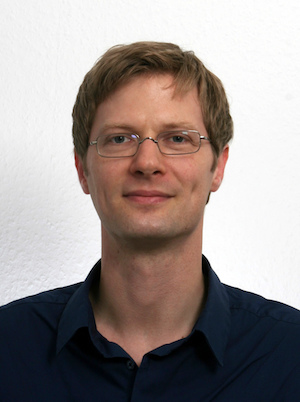
\includegraphics[width=0.32\textwidth]{images/liptow.jpg}
	\caption{Dr. Jasper Liptow. Quelle: \url{https://www.uni-frankfurt.de/45457854/liptow.jpg}}
	\label{fig:liptow}
\end{figure}

%\begin{figure}[h]
%	\centering
%	
\includegraphics[width=0.5\textwidth]{images/template.png}
%	\caption{Template Bild}
%	\label{fig:template}
%\end{figure}

\end{document}
